

\chapter{Desenvolvimento}
Nesta seção serão explicados os passos utilizados no desenvolvimento da interface de integração de chatbots em mais de um canal de comunicação. Os canais propostos inicialmente foram uma pagina web e o Slack. Além disso, O WhatsApp foi usando como canal complementar aos objetivos iniciais e forma de avaliar a dificuldade e o aspectos relacionados a possibilidade de estender o número de canais de comunicação.



\section{Desenvolvimento da Arquitetura}

Foi desenvolvido um chatbot composto por três componentes principais: Uma ou mais interface de comunicação com o usuário final (como Slack e paginas web), um componente de processamento de linguagem natural e um servidor webhook para gerenciar a troca de mensagens. 

Para processamento de linguagem natural foi utilizada a framework Rasa para mapear texto natural em dados estruturados como intenções e entidades bem como guiar o fluxo da conversa. O chatbot utilizado para integração possui um diálogo simples que busca identificar se um cliente em potencial possui interesse na compra e venda de determinados imóveis. Vale ressaltar que o  domínio em que se encontra o chatbot está fora do escopo deste trabalho.

\subsection{Webhooks}
Para que seja possível a integração de um agente conversacional, chatbot, em mais de um canal de comunicação é preciso que exista uma serviço que realize o gerenciamento das conversas e possa distribui-las em diferentes interfaces.

Webhooks, segundo a \citeonline{sendgrid2014webhook}, são uma forma de recebimento de informações, baseada em eventos, entre dois ou mais sistemas. Também chamado de \textit{Web callback}, em referência a funções ou rotinas que são executadas quando determinados eventos acontecem. Em suma,  webhooks são funções ou rotinas que são executadas quando notificadas da ocorrência de determinados eventos via HTTP (HyperText Transfer Protocol que em português significa Protocolo de Transferência de Hipertexto). Dessa forma, uma ação executada em um sistema A dispara uma ação em um sistema B.

O webhook também é chamado de API (Application Programming Interface que em português significa Interface de Programação de Aplicativos) reversa. Vale ressaltar que ambas abordagens possuem fatores comuns como o uso do protocolo HTTP e a implementação de funções ou rotinas definidas pelo usuário. A diferença é:

    \begin{itemize}
        \item Um webhook é baseado em eventos, ou seja, dois sistemas trocam informações e executam ações somente quando determinadas eventos acontecem.
        \item Uma API é guiada por requisições HTTP e, portanto, para um sistema A descobrir se determinado evento ocorreu em um sistema B precisaria realizar requisições frequentes para assim descobrir sobre o estado atual sistema B.  
    \end{itemize}

A figura \ref{fig:webhookdiff} ilustra a diferença fundamental entre as duas abordagens.

\begin{figure}[H]
  \centering
  \caption{Webhook X API ao longo do tempo.}
  \centering
  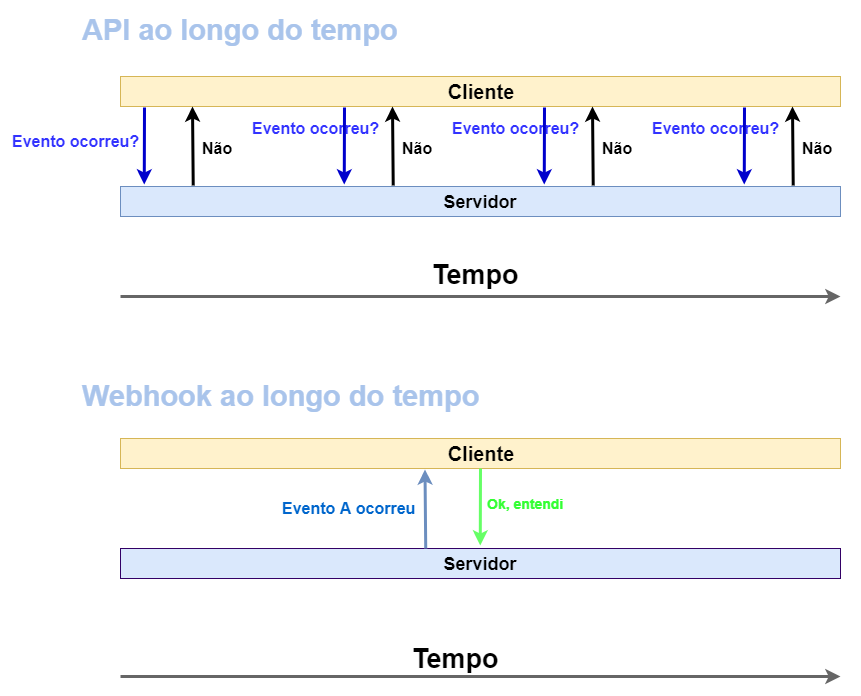
\includegraphics[scale=0.5]{Imagens/webhook-api.png} 
  \label{fig:webhookdiff}
  Fonte: O autor
\end{figure}



\textit{Webhooks}, são capazes de receber informações de sistemas externos sem uso desnecessário da rede e, portanto, foram utilizados para troca de mensagens entre os diferentes canais de comunicação. Assim, para desenvolver aplicações para Slack, Telegram,  Facebook Messenger e outros mensageiros é necessário a implementação de um servidor\textit{ webhook} que esteja esperando por eventos que são enviados pelos mensageiros para comunicação com cada plataforma. Na arquitetura proposta foi desenvolvido um único\textit{ webhook} que implementa a interface de API necessária para que o Slack, uma pagina web e o Whatsapp por meio do Twilio ser integrados com um chatbot.

Para a implementação do webhook foi necessário utilizar a documentação oficial da API do Slack e Twilio\footnote{https://www.twilio.com/} para estabelecer o padrão que deve ser esperado pelo webhook. Assim, Foi implementado um webhook capaz de comunicar-se com o Slack, uma página web e o Whatsapp. O Twilio é uma plataforma na nuvem que fornece chamadas telefônicas e mensagens de texto usando os webhooks e foi usado como um canal adicional neste trabalho.

Foi desenvolvido um servidor utilizando a \textit{framework Botkit} com um \textit{webhook} como interface de comunicação e um \textit{middleware} que realiza requisições (via protocolo http) para uma API de processamento de linguagem natural desenvolvida na framework Rasa. O conceito de middleware é utilizado na framework Botkit referenciando a funções que podem extender e personalizar funcionalidades padrão da framework. De acordo com a documentação oficial qualquer desenvolvedor pode criar seus próprios middlewares para modificar o comportamento da forma mais adequada ao projeto.

A partir disso, a arquitetura do chatbot foi elaborada levando em consideração um princípio da engenharia de software, a separação de interesses. A separação de interesses, de acordo com \citeonline{hursch1995separation} permite a localização de diferentes tipos de informações nos programas, facilitando o desenvolvimento, compreensão, reutilização e modificação. Para isso, cada componente, módulo ou camada do software deve ter uma função concisa cujo comportamento esperado, dado entrada e saída, é conhecido mas sua implementação não deve ser vista por componentes externos. A arquitetura proposta é ilustrada na figura \ref{fig:arquitetura} e o código principal que utiliza o middleware que se comunica com o módulo de processamento de linguaguem natural é apresentado na figura \ref{middleware-rasa}. 


\begin{figure}[H]
  \centering
   \caption{Arquitetura da framework de integração em multiplos canais}
  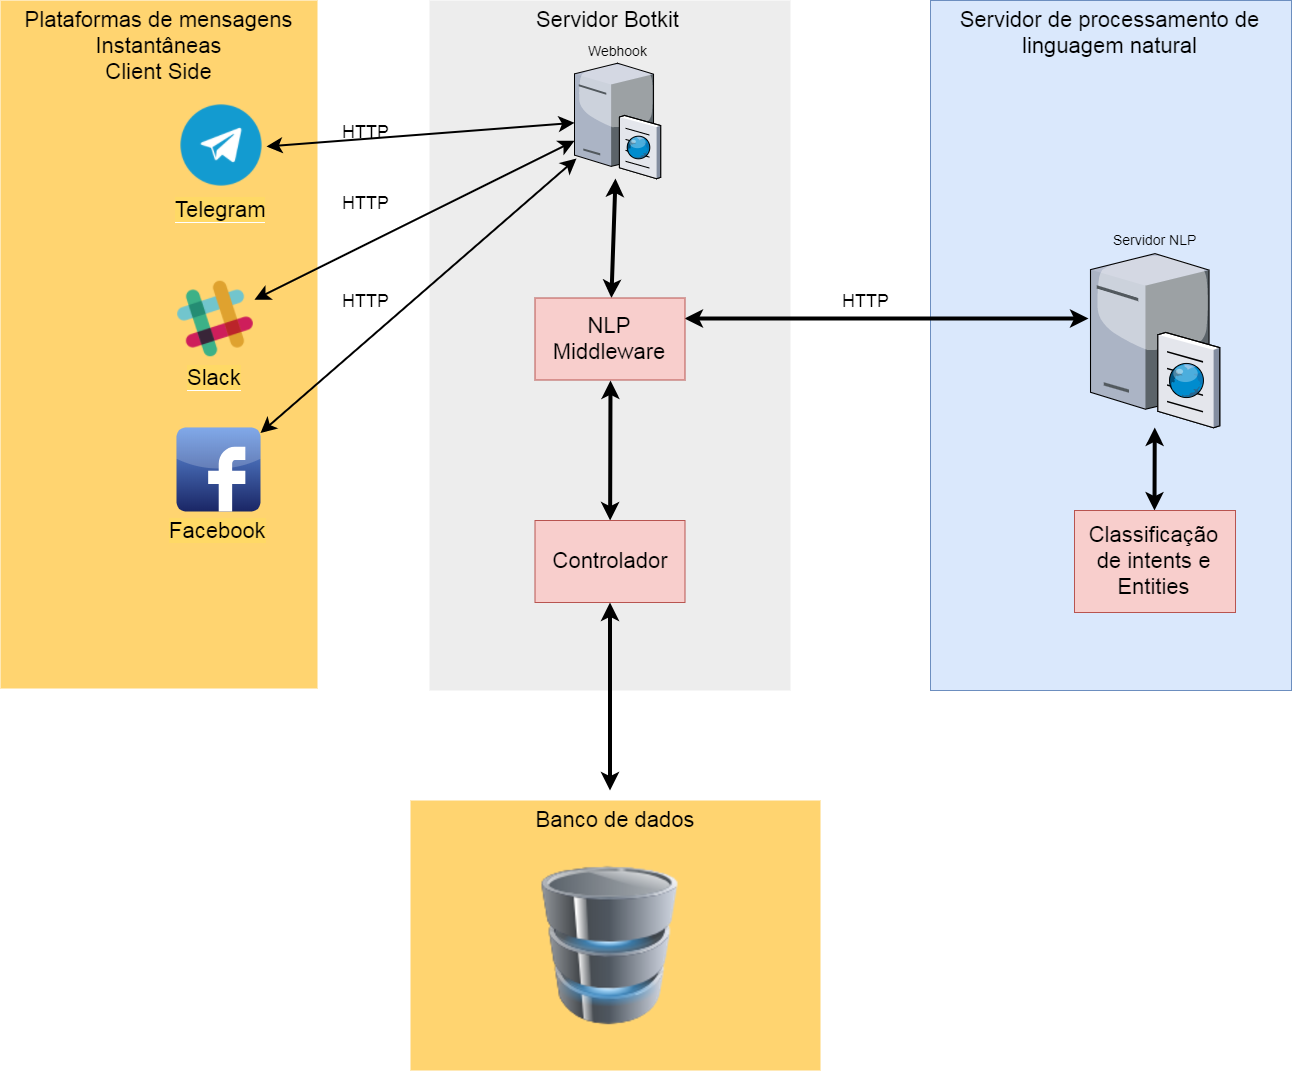
\includegraphics[scale=0.35]{Imagens/Botkit-architecture.png} 
  \label{fig:arquitetura}
  Fonte: O autor.
\end{figure}



\begin{figure}[H]
  \centering
   \caption{Código que utiliza o middleware NLP.}
  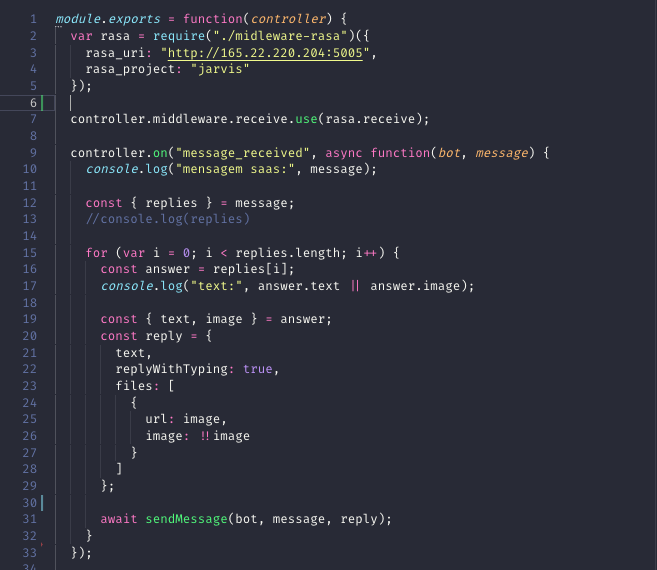
\includegraphics[scale=0.35]{Imagens/nlu-middleware.png} 
  \label{middleware-rasa}
  
\end{figure}


\subsection{Suporte ao protocolo HTTPS}

De acordo com \citeonline{naylor2014cost} o HTTPS é uma extensão segura do protocolo HTTP que utiliza uma camada de criptografia SSL/TLS, em inglês Secure Sockets Layer e Transport Layer Security, para estabelecer uma comunicação segura com o servidor. O SSL/TLS é essencial sempre que houver informações sensíveis sendo transmitidas, como nomes de usuário, senhas e informações de pagamento. 

Como webhooks são basicamente servidores é possível gerar o certificado junto a uma entidade verificada e garantir a autenticidade e segurança das mensagens que estão sendo trocadas. A integração com o Slack foi feita utilizando HTTPS porém nos outros canais foram utilizados somente HTTP.


\subsection{Implementação do Webhook}

O webhook é o intermediador entre o Slack, a pagina web, o whatsapp  e o chatbot. Sendo assim, ele fica esperando requisições HTTP, mais específicamente requisições feitas com o método POST, vindas dos canais de comunicação. A cada mensagem recebida, ele repassa a mensagem ao chatbot que, por sua vez, realiza determinadas ações e envia mensagens de resposta.

O webhook implementado executa em um servidor NodeJS e o mesmo utiliza uma porta para cada canal de comunicação presente na aplicação. Neste trabalho utilizamos três canais de comunicação, portanto, três portas foram usadas.

\subsubsection{Implementação do Webhook para o Slack}

O cérebro de uma aplicação que utiliza  a framework Botkit é chamado de controller (controlador em português).Um controller é uma interface que independe de plataformas e pode ser usado por desenvolvedores para adicionar recursos e funcionalidades ao chatbot. A figura \ref{fig:webhook_slack} mostra a utilização da instancia de um controller para configurar e gerenciar as requisições que serão recebidas do mensageiro Slack.

\begin{figure}[H]
  \centering
   \caption{Código principal do webhook esperando requisições do slack}
  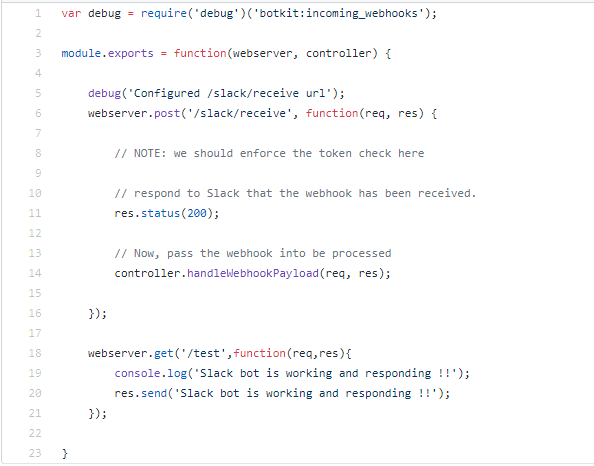
\includegraphics[scale=0.8]{Imagens/webhook_slack.png} 
  \label{fig:webhook_slack}
\end{figure}

\subsubsection{Implementação do Webhook para Web}

A implementação do chatbot na web difere dos mensageiros pois faz-se necessário a implementação de um script, executando no lado do cliente, que seja capaz de enviar requisições para o webhook que está no lado do servidor.

A framework Botkit fornece um script simples, juntamente com um layout html e css, que pode ser executado nos browsers que utiliza a arquitetura cliente-servidor. 

\begin{figure}[H]
  \centering
   \caption{Web Chat do Botkit que executa na arquitetura cliente-servidor  }
  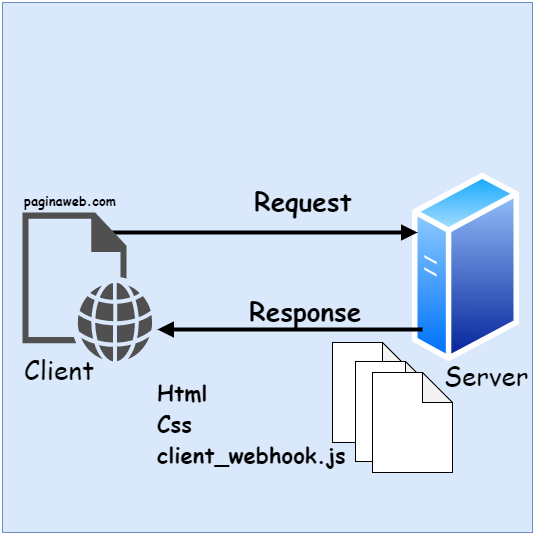
\includegraphics[scale=0.4]{Imagens/http-client.png} 
  \label{fig:http_webhook}
\end{figure}

A figura \ref{fig:http_webhook} mostra como acontece a comunicação cliente-servidor e a renderização da interface do chat juntamento com o script que executa no lado cliente. No Slack, e em outros mensageiros, todos os eventos relacionados a interação entre o usuário e o chatbot são enviados automáticamente para o webhook que definimos.

Na web, o script que executa nos browsers fica aguandando mensagens do usuário e as repassa via http para o webhook do lado do servidor. As figuras \ref{fig:webhook_deliver} e \ref{fig:webhook_code} mostram os códigos responsáveis por essas tarefas. 

\begin{figure}[H]
  \centering
   \caption{Código executado quando o usuário digita uma mensagem}
  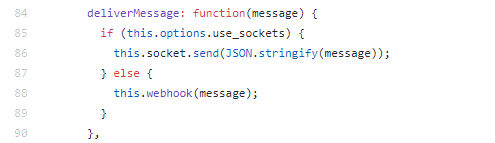
\includegraphics[scale=0.8]{Imagens/deliver_webhook.png} 
  \label{fig:webhook_deliver}
\end{figure}


\begin{figure}[H]
  \centering
   \caption{Código responsável pela comunicação entre cliente-servidor}
  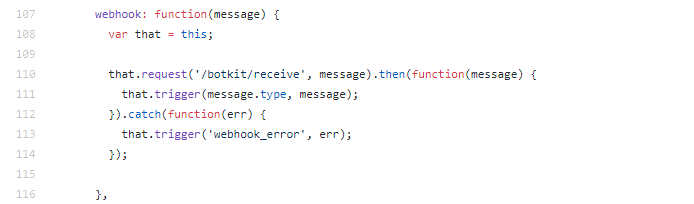
\includegraphics[scale=0.8]{Imagens/webhook_code.png} 
  \label{fig:webhook_code}
\end{figure}


\subsubsection{Formas de utilizar o chatbot na Web}

È importante destacar que a estrutura inicial que o Botkit oferece pode e deve ser customizada para atender aos requisitos do projeto a ser desenvolvido. Além disso, existem três maneira que desenvolvedores podem utilizar o botkit na web:

\begin{itemize}
    \item Iframes com paginas embutidas
    \item Link direto para uma pagina do chatbot
    \item Embutir a interface do chat em uma pagina web existente
\end{itemize}


\begin{figure}[H]
  \centering
   \caption{Código para embutir chatbot em um iframe}
  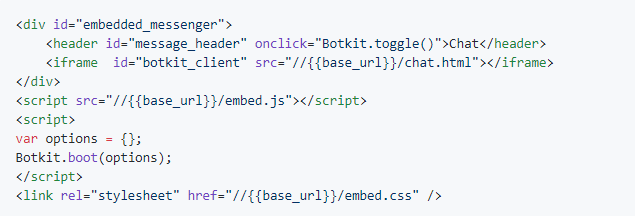
\includegraphics[scale=0.8]{Imagens/iframe.png} 
  \label{iframe}
\end{figure}

O código ilustrado na figura \ref{iframe} é um exemplo de como desenvolvedores podem embutir o chat no lado cliente utilizando a tag iframe do html. Os outros casos de uso requerem habilidades de programação web mas são bem simples.

Em suma, desenvolvedores também podem hospedar diretamente todos os arquivos do chat e obter um domínio que direcione para o chatbot ou inserir os arquivos html, css e javascript diretamente em uma pagina web já existente. A figura \ref{chatweb} ilustra a interface inicial do chatbot na web.


\begin{figure}[H]
  \caption{Interface web do chatbot web.}
  \centering
  
  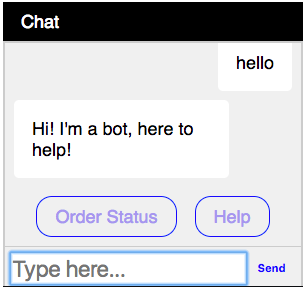
\includegraphics[scale=0.8]{Imagens/chat-exemple.png} 
   \caption{Fonte: Botkit}
  \label{chatweb}
\end{figure}



\section{Integração Com o Slack}

Em 2015 a framework Botkit foi comprada pela Microsoft e alguns serviços foram Migrados para o Microsoft Bot Framework. Essa framework que fica hospedada nos servidores da Microsoft facilita a criação de um único bot que pode ser executado em vários canais de mensagens, incluindo Skype, Group.me, Facebook Messenger, Slack, Telegram, Kik, SMS e e-mail.

Entretanto, para este trabalho soluções hospedadas e pagas não poderiam ser levadas em consideração. Na documentação oficial do Botkit é recomendado que se utilize a framework da Microsoft para integrações com Telegram e outros canais de comunicação.

Devido essa limitação do Botkit não foi possível utilizar o Telegram como canal de comunicação e o Slack foi selecionado. Entretanto, por ser um projeto open source é possível desenvolver um middleware que funcione com o telegram e outros canais em nodejs. 

\subsection{Criando Aplicação na API do Slack}

Para integrar um bot na plataforma do Slack é necessário criar uma conta de desenvolvedor na API oficial\footnote{https://api.slack.com/tutorials}. No Slack, um bot é controlado programaticamente por meio de um token de usuário de bot que tem acesso a uma ou mais APIs do Slack. Além disso, um bot para o slack é uma aplicação que precisa ser criada conforme a figura \ref{cadastro_slack}.

\begin{figure}[H]
  \centering
   \caption{Criando uma aplicação na API do Slack}
  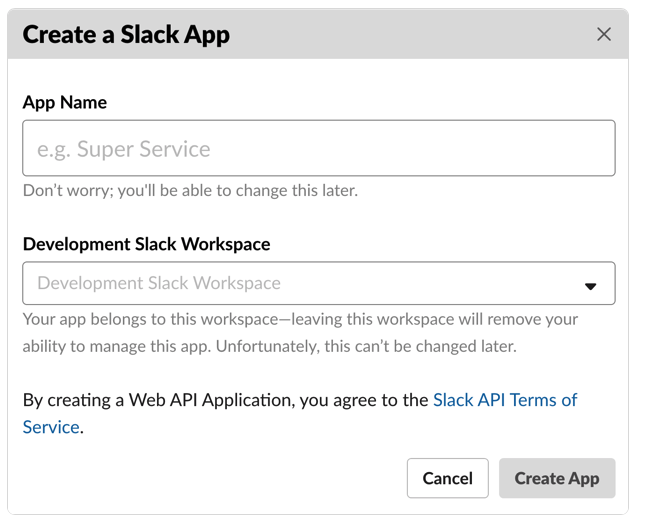
\includegraphics[scale=0.5]{Imagens/slack_cadastro.png} 
  \label{cadastro_slack}
\end{figure}

Assim que a aplicação é criada e autorizada a executar no Slack, as credenciais de seguranças estarão disponíveis. A partir disso, é necessário pegar as credenciais geradas e utiliza-las para inicializar o chatbot como ilustram as figuras \ref{token} e \ref{token_codigo}.

\begin{figure}[H]
  \centering
   \caption{Credenciais de segurançã da API do Slack}
  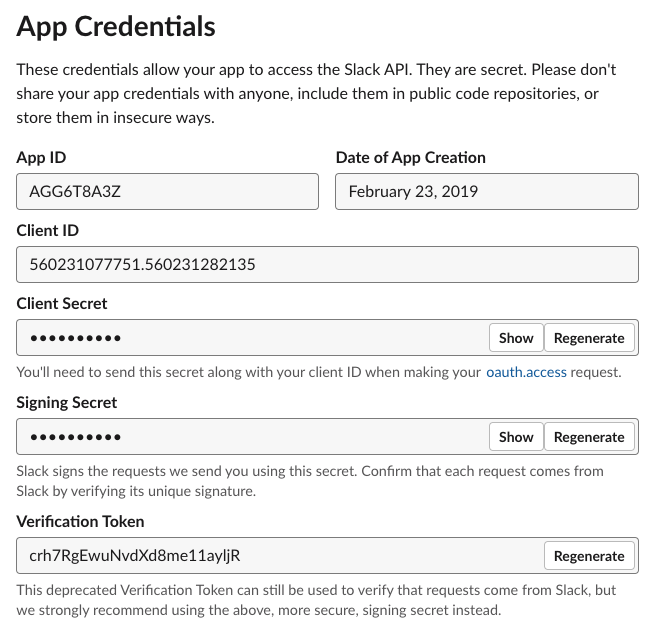
\includegraphics[scale=0.5]{Imagens/slack_token.png} 
  \label{token}
\end{figure}



\begin{figure}[H]
  \centering
   \caption{Código responsável por inicializar o chatbot com as credenciais do Slack}
  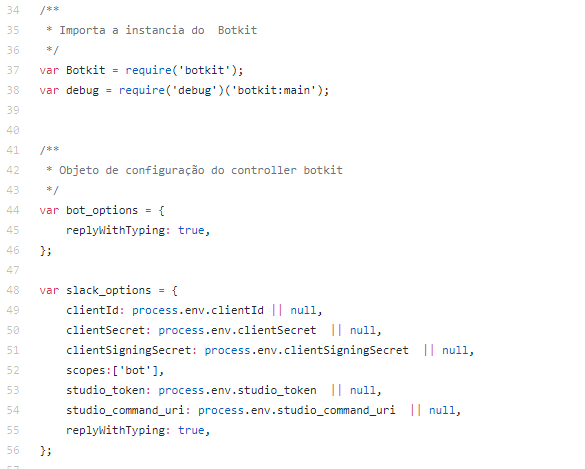
\includegraphics[scale=0.8]{Imagens/config.png} 
  \label{token_codigo}
\end{figure}



\begin{figure}[H]
  \centering
   \caption{Código responsável por inicializar o chatbot com as credenciais do Slack}
  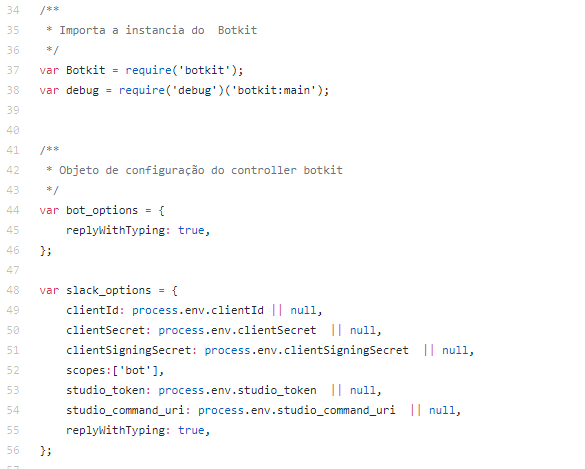
\includegraphics[scale=0.8]{Imagens/config.png} 
  \label{token_codigo}
\end{figure}



Após a obtenção das credenciais que serão usadas para integrar o chatbot no mensageiro configurar a URL do webhook onde serão enviadas as notificações dos eventos. Essa configuração é ilustrada na figura \ref{webhook-slack-config}. Uma vez que essa configuração foi realizada, o slack irá enviar alguns eventos de teste para o servidor webhook que está no endereço fornecido para confirmar o funcionamento da aplicação. Dessa forma, o código responsável por responder os eventos emitidos pelo slack é apresentado na figura X. 


\begin{figure}[H]
  \centering
   \caption{Configuração da URL do webhook.}
  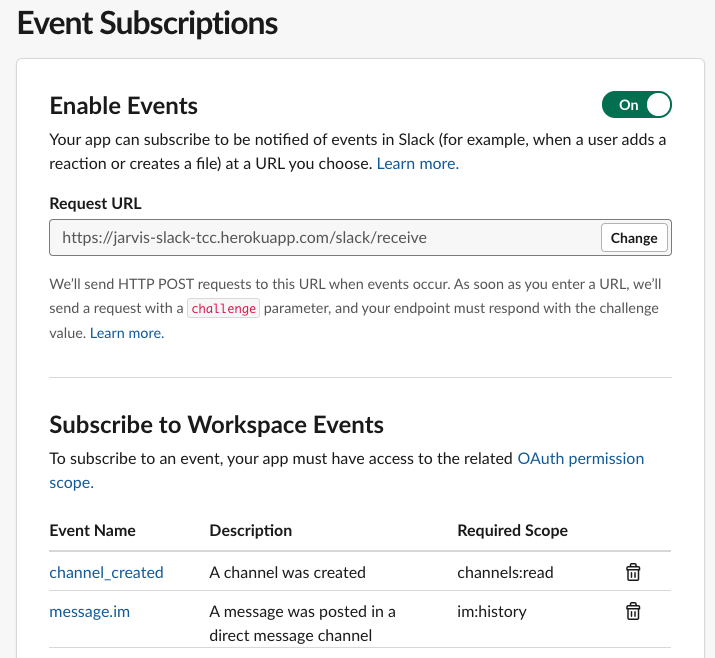
\includegraphics[scale=0.5]{Imagens/Slack_webhook_app.png} 
  \label{webhook-slack-config}
\end{figure}


\begin{figure}[H]
  \centering
   \caption{Código responsável por receber eventos do slack.}
  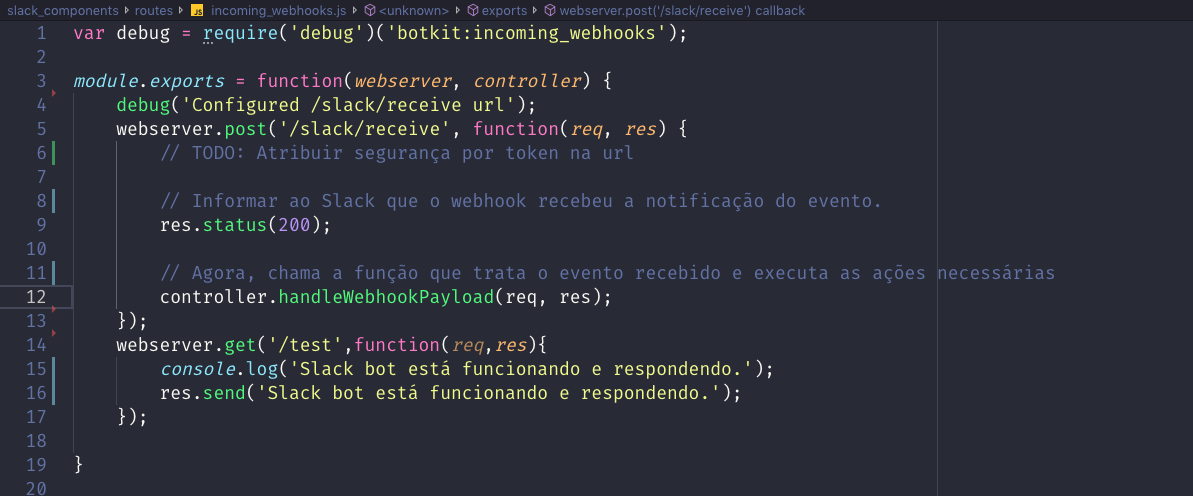
\includegraphics[scale=0.3]{Imagens/webhook-code-slack.png} 
  \label{webhook-slack-config}
\end{figure}




\section{Implantação do Servidor}

Para que o servidor webhook consiga gerenciar as requisições vindas de vários canais, é imprescindível que ele esteja disponível na internet. Sendo assim, para a fase de implantação na web foi utilizado o Heroku\footnote{https://www.heroku.com} e Digital Ocean para hospedar o servidor na nuvem. 

O Heroku é uma plataforma em nuvem como um serviço que suporta várias linguagens de programação. As principais linguagens suportadas são Java, Node.js, Scala, Clojure, Python, PHP e Go. Essa plataforma possui um plano gratuito para desenvolvedores e, portanto, atende as necessidades deste trabalho.

O digital Ocean é um provedor americano de infraestrutura de nuvem com sede em Nova York e data centers em todo o mundo. Sendo assim, foi utilizada uma máquina virtual linux hospedada do digital ocean.

Uma combinação das duas plataformas (Heroku e Digital ocean) foi utilizada pelo fato de que o uso da API do Slack necessita de conexões que utilizam o conexões seguras por meio do protocolo HTTPS. Assim, Após a implantação do código na nuvem, o Heroku disponibiliza uma URL \footnote{Uniform Resource Locator que em português significa "localizador uniforme de recursos". Esse termo se refere ao endereço de rede no qual se encontra algum recurso computacional} que torna público os serviços implementados no servidor webhook e que possui certificado de segurança SSL (\textit{Secure Sockets Layer}) válido. 

Portanto, no servidor digital ocean foi hospedado a maior parte dos serviços que não necessitam de conexão HTTPS e a integração segura com o Slack foi hospedada no Heroku.

O servidor webhook e a interface web do chatbot está disponível na url: \url{https://jarvis-bot-tcc.herokuapp.com}.



\subsection{Integração com Twilio/Whatsapp}

Para que o chatbot fosse capaz de comunicar-se por meio do mensageiro whatsapp foi utilizada a plataforma Twilio. Essa plataforma  quee possibilita que desenvolvedores de software integrem voz, mensagens de texto, video, notificações e facilidades de comunicação em  geral em seus aplicativos. Essa integração pode ser feita usando API ou webhook.

O twilio disponibiliza um ambiente de testes, também chamado de sandbox, onde o desenvolvedor configura uma URL para recebimento de eventos. Dessa forma, quando um usuário envia uma mensagem no whatsapp para um número definido o webhook do twilio dispara esse evento, juntamente com a mensagem, para a URL definida pelo desenvolvedor. O twilio utiliza a API do whatsapp \footnote{https://www.whatsapp.com/business/api}, em inglês Whatsapp Business API, para troca de informações e eventos com o mensageiro.

Vale ressaltar que o facebook, empresa que mantém o whatsapp, limita o uso da API para que somente empresas verificadas tenham acesso. O twilio, portanto, é uma plataforma autorizada e é atualmente o principal meio de comunicação programável com o mensageiro.

Sendo assim, uma conta no twilio foi criada e configurada realizar a integração com o whatsapp. De acordo com a documentação oficial do twilio, é necessário criar um projeto, configurar a URL do webhook e obter as credenciais de acesso como mostras as figuras \ref{twilio-project}, \ref{url-twilio} e \ref{twilio-tokens} respectivamente. 



\begin{figure}[H]
  \centering
   \caption{Criação de um projeto na plataforma twilio.}
  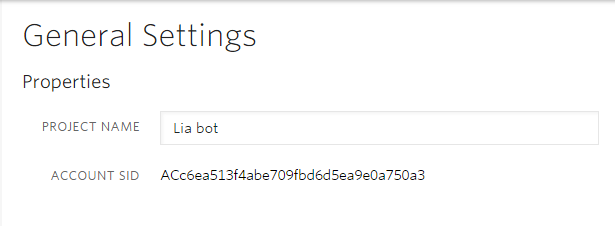
\includegraphics[scale=0.5]{Imagens/twilioproject.PNG} 
  \label{twilio-project}
\end{figure}


\begin{figure}[H]
  \centering
   \caption{Configurando a URL do webhook.}
  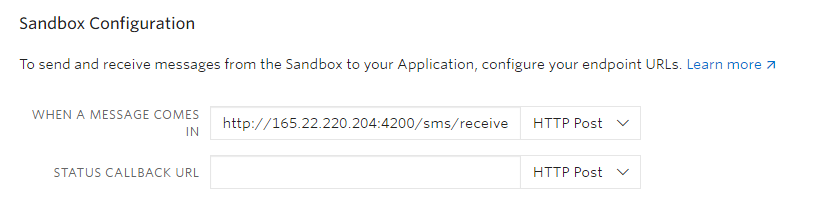
\includegraphics[scale=0.5]{Imagens/urlcallback.PNG} 
  \label{url-twilio}
\end{figure}



\begin{figure}[H]
  \centering
   \caption{Credenciais de acesso geradas pelo twilio.}
  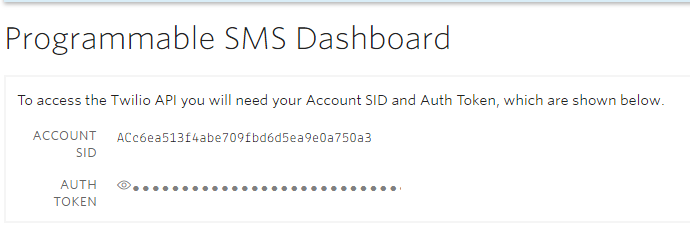
\includegraphics[scale=0.5]{Imagens/tokentwilio.PNG} 
  \label{twilio-tokens}
\end{figure}


Após a configuração da URL como ilutra a figura \ref{url-twilio} foi o webhook foi configurado para atender requisições HTTP nessa URL como mostra as figura \ref{twilio-tokens-code} e \ref{twilio-webhook-code}.


\begin{figure}[H]
  \centering
   \caption{Código responsável por configurar as credenciais de acesso ao twilio.}
  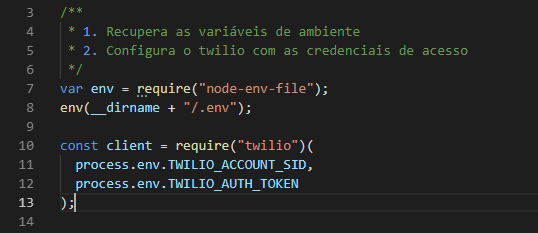
\includegraphics[scale=0.5]{Imagens/twilio-credenciais.PNG} 
  \label{twilio-tokens-code}
\end{figure}


\begin{figure}[H]
  \centering
   \caption{Código responsável por configurar o webhook para receber eventos do twilio}
  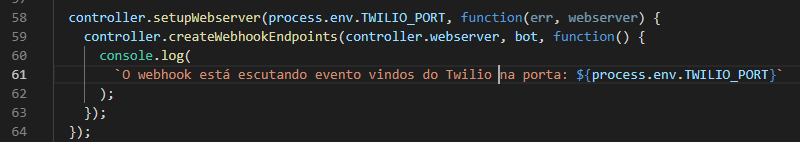
\includegraphics[scale=0.5]{Imagens/twilio-webhook-code.PNG} 
  \label{twilio-webhook-code}
\end{figure}






\chapter{Resultados }

Nesta Seção são apresentados os resultados obtidos com a implantação de um ambiente de trabalho para o funcionamento do chatbot em uma pagina web, slack e whatsapp. A integração permitiu que o chatbot, chamado de lia, pudesse estar presente em todos os canais propostos e exemplos de conversas nesses canais são ilustrados.

\section{Conversa com o chatbot no Slack}

O slack é uma plataforma de comunicação principalmente para empresas, abrangente e com funcionalidades que lembram um chat que também faz chamadas em vídeo, só que com muito mais capacidade de customização e interação entre os participantes, além de comandos ágeis e facilidade para compartilhar os mais diversos tipos de arquivos. Nesse mensageiro é possível:


\begin{itemize}
    \item Criar times: Um time normalmente será por onde você gerenciará a comunicação interna de sua empresa, por exemplo. É possível criar mais de um time caso sua empresa seja dividida em unidades de negócios, como diretoria de marketing e vendas.

    \item Criar canais: Para cada time você cria canais com seus assuntos de interesse. Por exemplo: criação, atendimento ao cliente, produção, desenvolvimento, suporte etc. Esses canais podem ser públicos, com acesso de todos os participantes da empresa, ou fechados.

    \item Enviar Mensagens diretas: Quer falar diretamente com alguém? Você pode trocar mensagens diretamente com uma pessoa ou grupo sem que o canal inteiro participe e não precisa recorrer ao WhatsApp.

    \item Executar Comandos Slash: O Slack tem uma série de comandos para facilitar sua vida. Por exemplo, se quer citar uma pessoa, use '@nomedapessoa', ou se quer notificar um canal, use '#nomedocanal', quando estiver digitando sua mensagem.
\end{itemize}

Portanto, uma vez realizada a integração com o slack o chatbot pode se comunicar por meio de times, canais, mensagens diretas e outros comandas existentes.  As figuras \ref{slack01} e \ref{slack02} mostram uma conversa com o chatbot por meio de mensagens diretas e a figura \ref{slack03} mostra o chatbot respondendo a uma citação.


\begin{figure}[H]
  \centering
   \caption{Mensagem direta com o chatbot no slack.}
  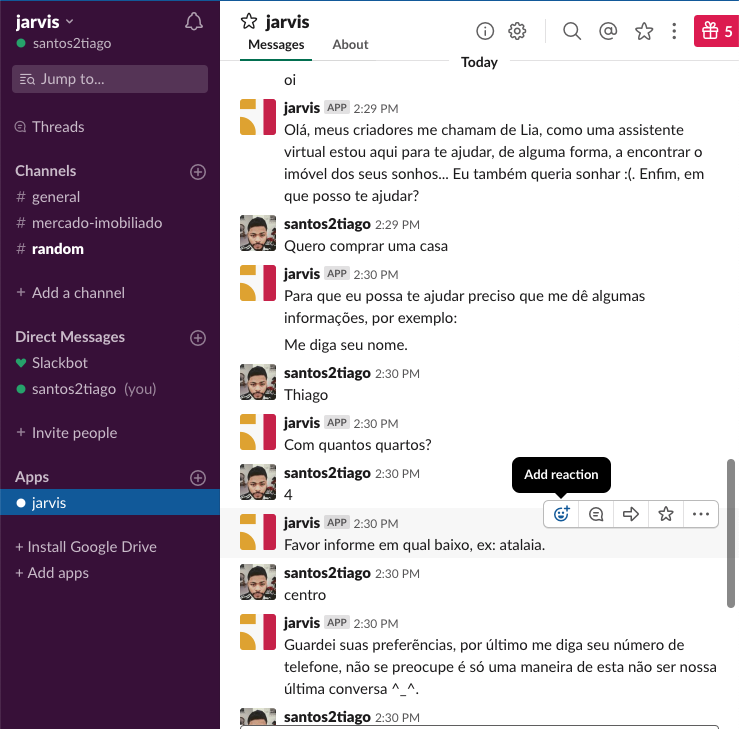
\includegraphics[scale=0.5]{Imagens/slack01.png} 
  \label{slack01}
\end{figure}


\begin{figure}[H]
  \centering
   \caption{Mensagem direta com o chatbot no slack.}
  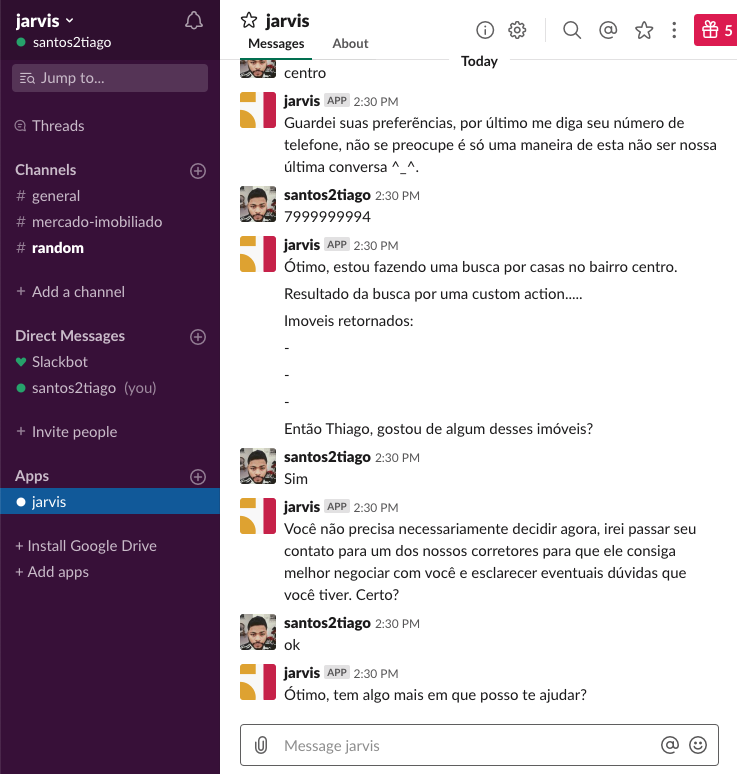
\includegraphics[scale=0.5]{Imagens/slack02.png} 
  \label{slack02}
\end{figure}



\begin{figure}[H]
  \centering
   \caption{Conversa com o chatbot por citação no slack.}
  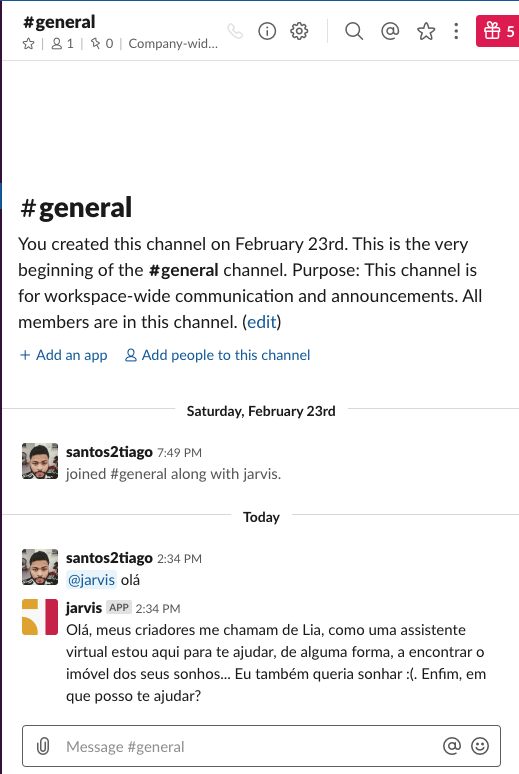
\includegraphics[scale=0.5]{Imagens/slack03.png} 
  \label{slack03}
\end{figure}

\section{Conversa com o chatbot na Web}

Para iniciar uma conversa com o chatbot na web basta acessar a URL a seguir:

\begin{itemize}
    \item http//165.22.220.204:8443/chat.html
\end{itemize}


\begin{figure}[H]
  \centering
   \caption{Iniciando conversa com o chatbot na web.}
  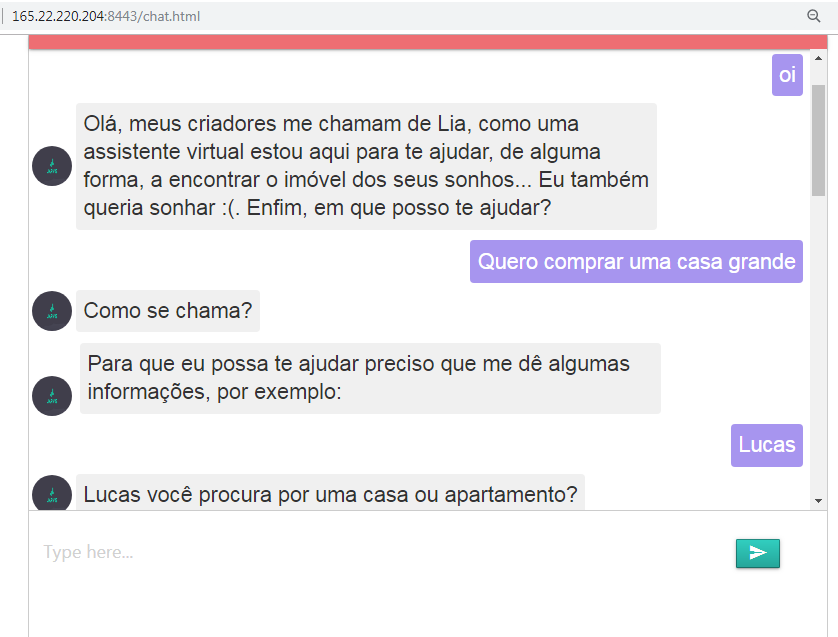
\includegraphics[scale=0.5]{Imagens/chat1.PNG} 
  \label{twilio-webhook-code}
\end{figure}

\begin{figure}[H]
  \centering
   \caption{conversa com o chatbot.}
  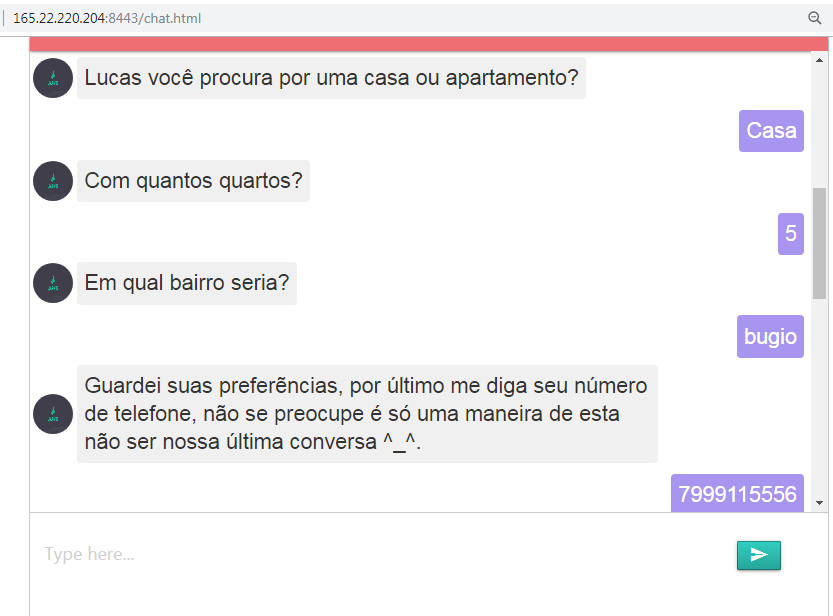
\includegraphics[scale=0.5]{Imagens/chat2.PNG} 
  \label{twilio-webhook-code}
\end{figure}

\begin{figure}[H]
  \centering
   \caption{conversa com o chatbot.}
  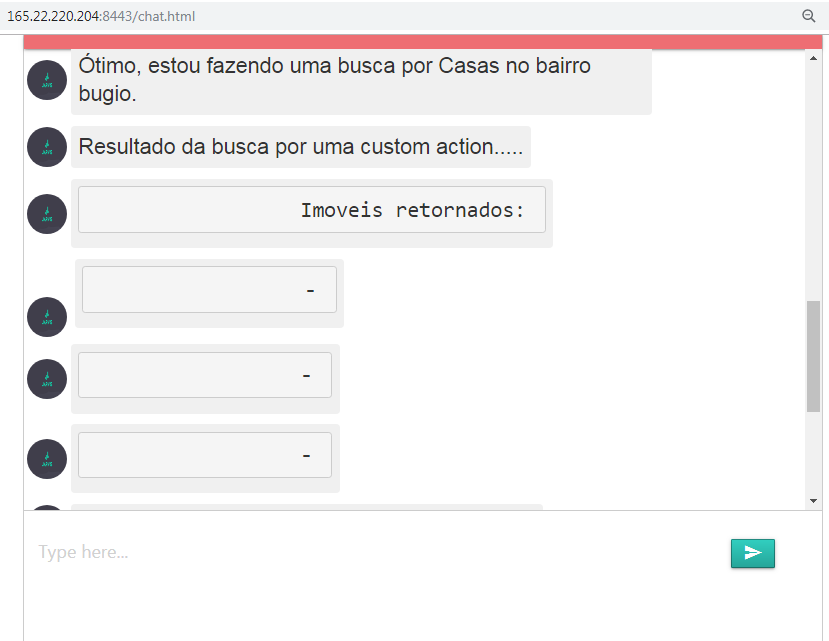
\includegraphics[scale=0.5]{Imagens/chat3.PNG} 
  \label{twilio-webhook-code}
\end{figure}



\section{Conversa com o chatbot no Whatsapp}

O ambiente de desenvolvimento do twilio, chamado de sandbox, possui três números de telefone pré-configurados como contas comerciais do whatsapp e são compartilhados entre todos os usuários do sandbox. Para usar o Sandbox, você deve começar optando pelo sandbox enviando o número de telefone que escolheu uma mensagem do WhatsApp. Uma vez ativado, você receberá apenas mensagens da sua Sandbox específica. A configuração da sendbox para este trabalho está ilustrada na figura \ref{twilio-sandbox}.


\begin{figure}[H]
  \centering
   \caption{Configurando o sandbox do twilio entrar no canal de comunicação do chatbot.}
  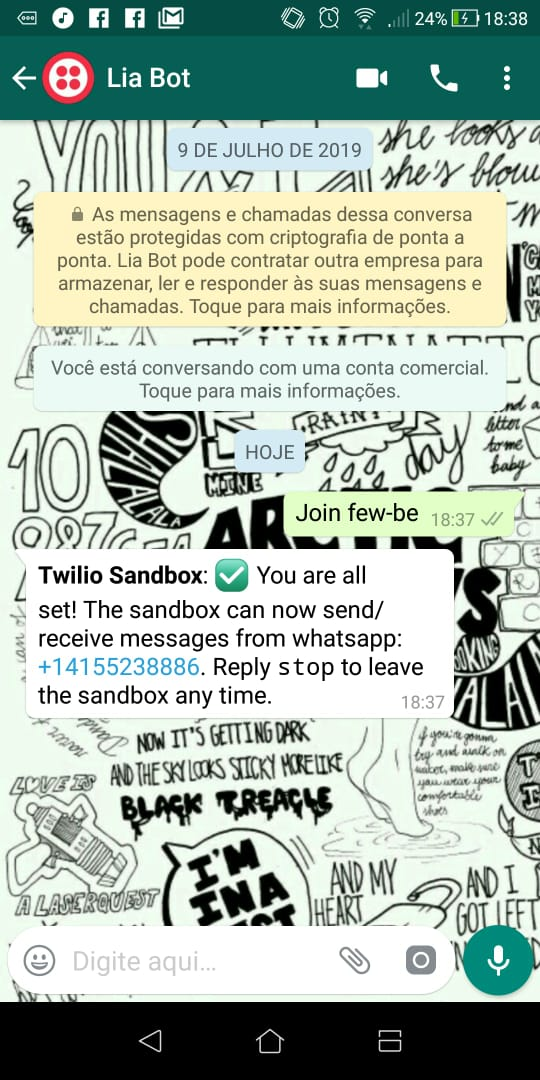
\includegraphics[scale=0.35]{Imagens/twilio-sandbox.jpeg} 
  \label{twilio-sandbox}
\end{figure}


Uma vez configurado o ambiente de desenvolvimento, o sandbox, é possível conversar normalmente com o chatbot. As figura \ref{twilio-conversa1}, \ref{twilio-conversa2}, e \ref{twilio-conversa3} mostram um exemplo de diálogo.


\begin{figure}[H]
  \centering
   \caption{Conversando com o chatbot no whatsapp.}
  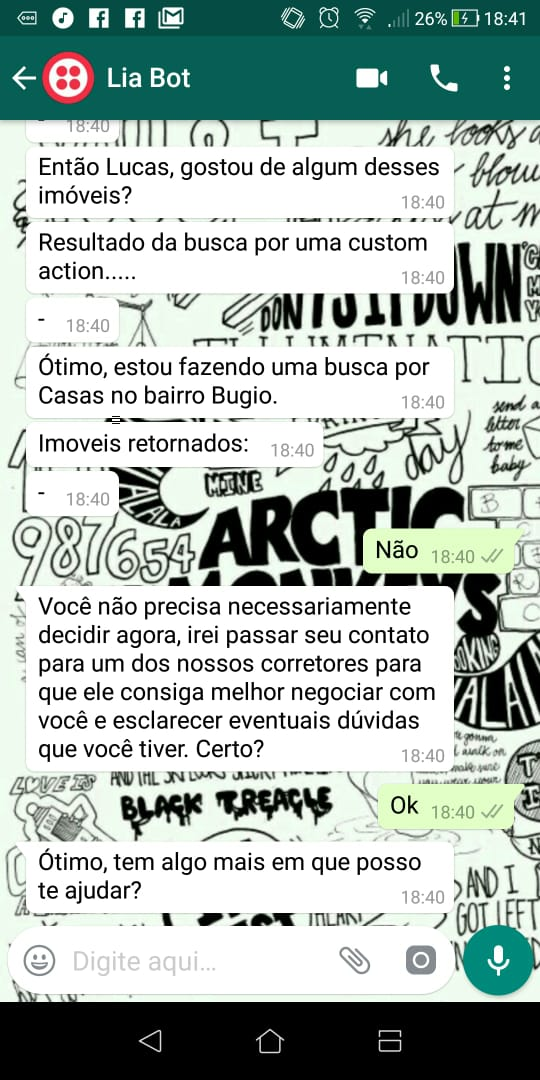
\includegraphics[scale=0.5]{Imagens/twilio-conversa1.jpeg} 
  \label{twilio-conversa1}
\end{figure}

\begin{figure}[H]
  \centering
   \caption{Conversando com o chatbot no whatsapp}
  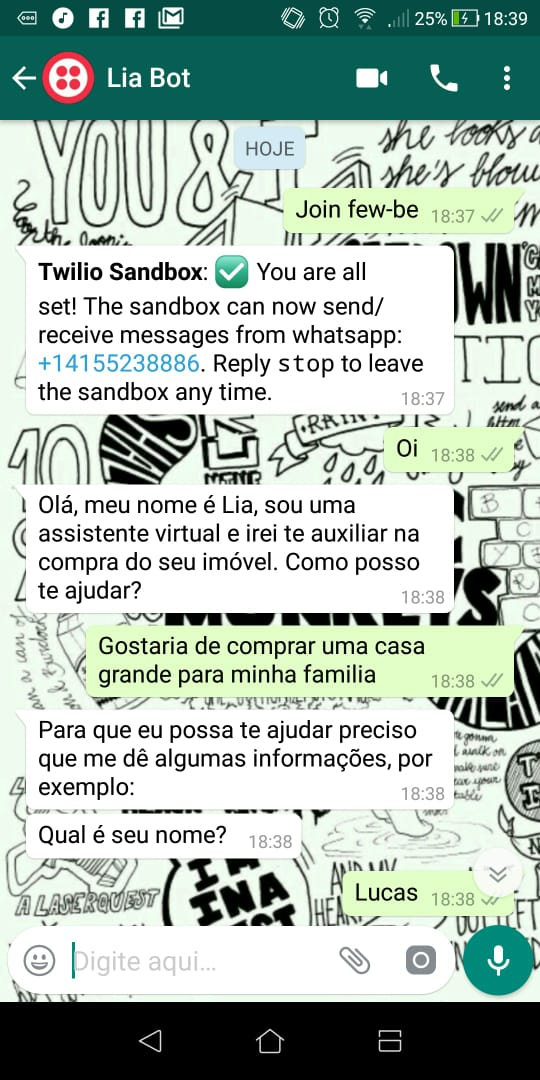
\includegraphics[scale=0.5]{Imagens/twilio-conversa2.jpeg} 
  \label{twilio-conversa2}
\end{figure}


\subsection{Extensão da integração}

A partir da definição da arquitetura modular e com partes que possuem funções coesas foi possível realizar a extensão da integração em mais um canal, o Whatsapp. Assim, uma vez que a base de conhecimento ou cérebro do chatbot está em funcionamento de acordo com a arquitetura é possível, com algumas modificações no conector, realizar a integração em outros canais. 

Vale destacar que a proposta de integração deste trabalho é flexível e não necessariamente precisa ser adotada para o desenvolvimento de chatbots. Entretanto, a arquitetura modularizada e coesa, um artefato gerado neste trabalho, deve ser adotada para evitar um alto acoplamento que pode causar problemas para evoluir o software.

De maneira geral, para adição de novos canais é necessário o entendimento da arquitetura e configuração de uma nova URL para o webhook do servidor no canal pretendido.


\subsection{Validação}

A validação do chatbot foi realizada em duas etapas. Em um primeiro momento foi feito um teste automatizado do servidor webhook, sendo que foi utilizada uma ferramenta que realiza testes por meio de requisições HTTP e exibe os resultados obtidos bem como o sucesso o falha do teste. Após essa primeira validação, o chatbot foi submetido a testes de estresse também com o uso de uma ferramenta de automatização de testes.


\subsubsection{Tarefa um de validação}
Neste passo foi utilizada a ferramenta online API TESTER\footnote{https://apitester.com/} onde é possível Fazer solicitações HTTP, extrair valores das respostas, verificar que os valores estão corretos, separar os testes por etapas, reutilizar variáveis nas etapas ou criar lógica customizada usando JavaScript. Portanto, um teste com quatro passos foi construído para validar e verificar que o servidor webhook está funcionando e respondendo adequadamente as mensagens dos usuários.

Com essa ferramenta é possível criar um teste com vários passos e, portanto, o teste criado foi dividido em quatro passos e tem o objetivo exclusivo de  verificar se a integração foi bem sucedida e está respondendo e atendendo as requisições dos usuários. Esse teste não tem o objetivo de cobrir todas as possibilidades de conversas entre o chatbot e o usuário mas verificar se a integração está funcional. Ou seja, o teste tem o intuito de verificar se para casa mensagem enviada no lado cliente existe uma resposta do chatbot.


\begin{figure}[H]
  \centering
   \caption{Passo um: Verifica se o servidor está online e funcionando.}
  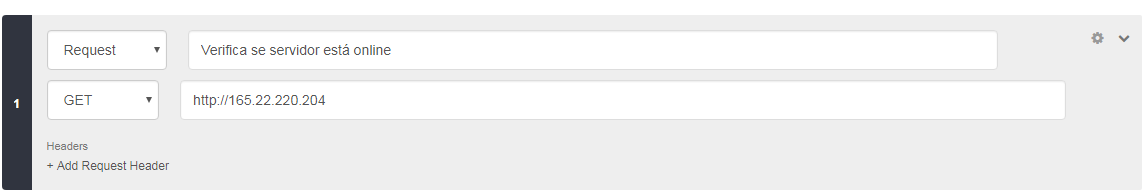
\includegraphics[scale=0.5]{Imagens/passo1.PNG} 
  \label{teste1}
\end{figure}

\begin{figure}[H]
  \centering
   \caption{Passo dois: Simula um usuário cumprimentando o chatbot.}
  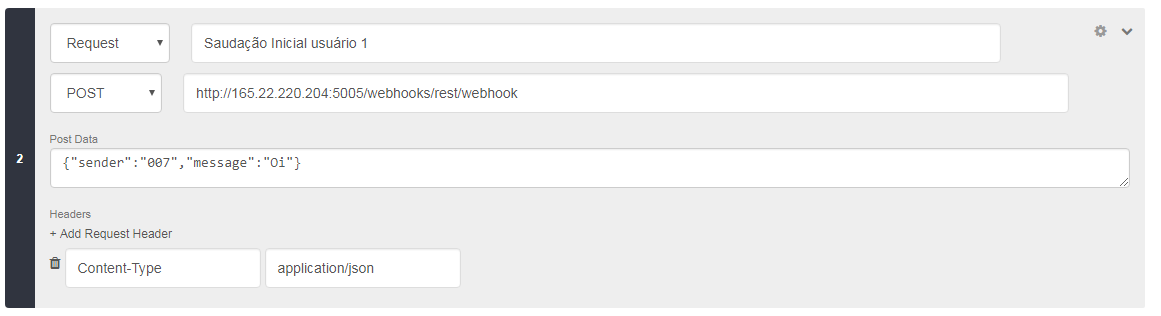
\includegraphics[scale=0.5]{Imagens/passo2.PNG} 
  \label{teste2}
\end{figure}

\begin{figure}[H]
  \centering
   \caption{Passo três: Simula outro usuário cumprimentando o chatbot.}
  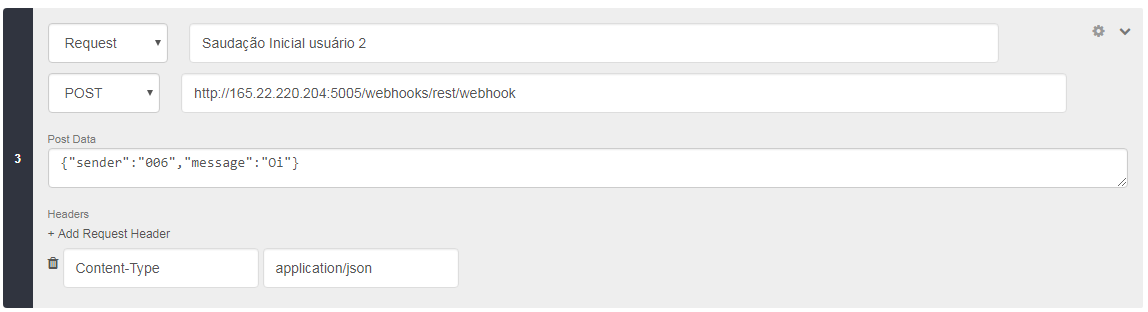
\includegraphics[scale=0.5]{Imagens/passo3.PNG} 
  \label{teste3}
\end{figure}

\begin{figure}[H]
  \centering
   \caption{Passo quatro: Simula um usuário com intençao de comprar um imóvel.}
  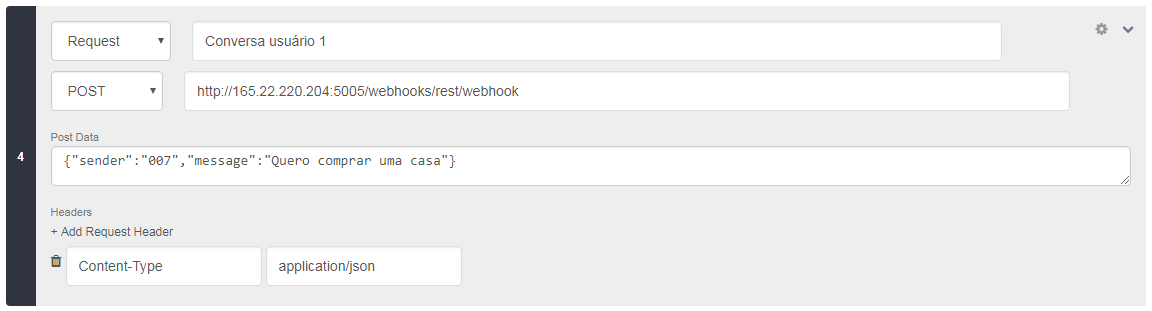
\includegraphics[scale=0.5]{Imagens/passo4.PNG} 
  \label{teste4}
\end{figure}

Após a execução do teste verificou-se que todos quatro passos obtiveram sucesso e a integração foi bem sucedida. as figuras \ref{resultado-teste1}, \ref{resultado-teste2}, \ref{resultado-teste3} e \ref{resultado-teste4} mostram o resultado obtido após a execução do teste.

\begin{figure}[H]
  \centering
   \caption{Resultado do passo um.}
  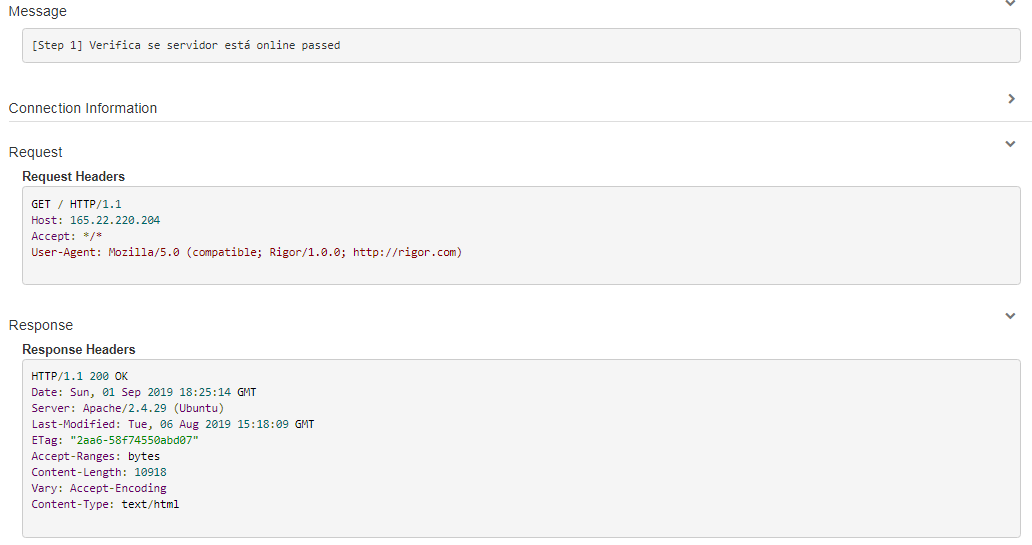
\includegraphics[scale=0.5]{Imagens/resultado1.PNG} 
  \label{resultado-teste1}
\end{figure}


\begin{figure}[H]
  \centering
   \caption{Resultado do passo dois.}
  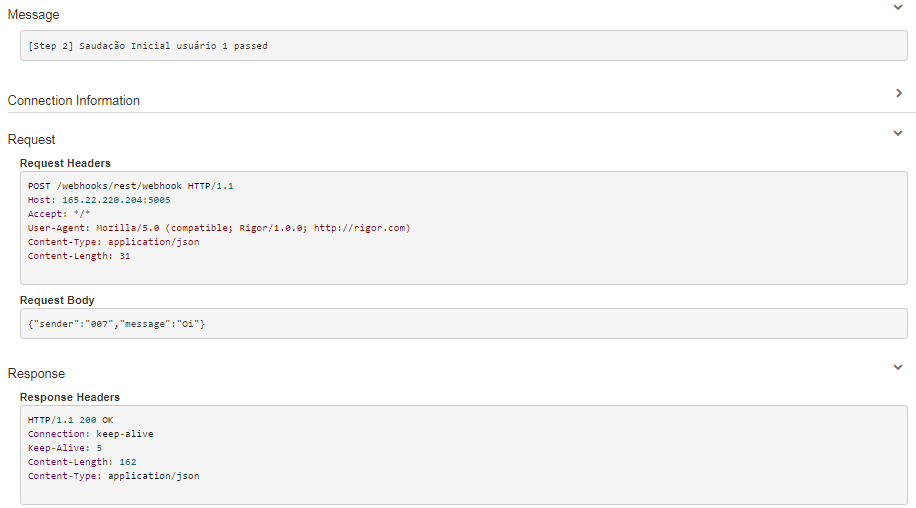
\includegraphics[scale=0.5]{Imagens/resultado2.PNG} 
  \label{resultado-teste2}
\end{figure}


\begin{figure}[H]
  \centering
   \caption{Resultado do passo três.}
  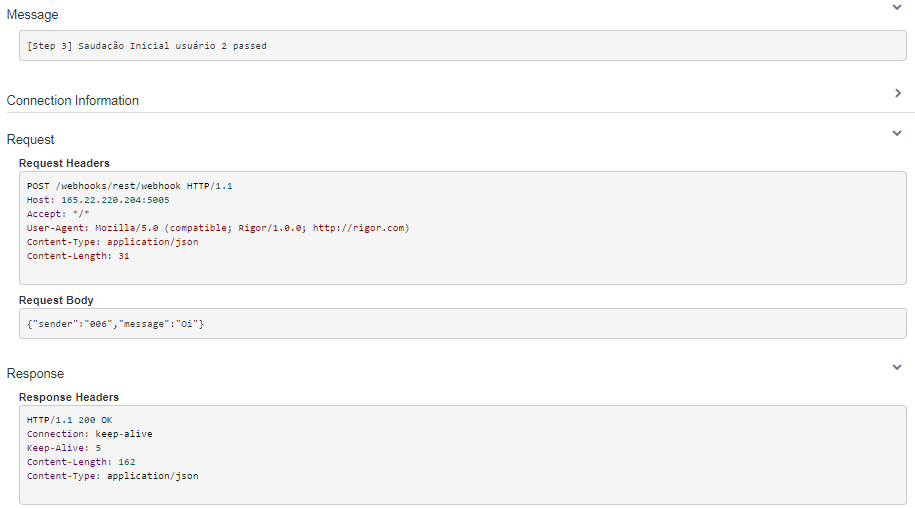
\includegraphics[scale=0.5]{Imagens/resutado3.PNG} 
  \label{resultado-teste3}
\end{figure}


\begin{figure}[H]
  \centering
   \caption{Resultado do passo quatro.}
  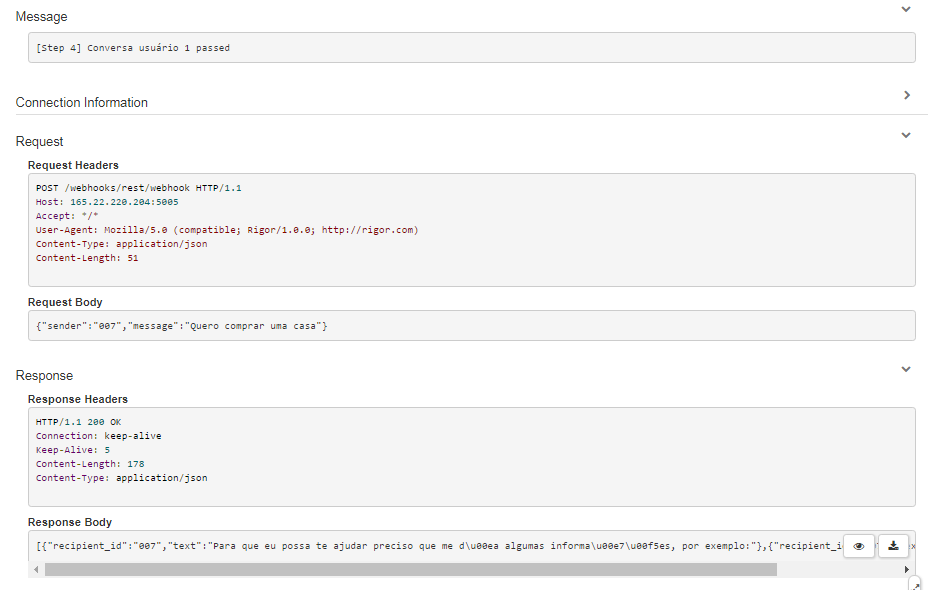
\includegraphics[scale=0.5]{Imagens/resultado4.PNG} 
  \label{resultado-teste4}
\end{figure}


\subsubsection{Tarefa dois de validação}
Neste passo foi utilizada a ferramenta online RESTFUL STRESS\footnote{https://chrome.google.com/webstore/detail/restful-stress/lljgneahfmgjmpglpbhmkangancgdgeb} onde é possível realizar testes de estresse por meio do protocolo HTTP e verificar que os valores estão corretos de acordo com o número de requisições definidas. A ferramenta disponibiliza gráficos com os resultados dos testes.

Um teste de estresse é realizado para submeter o software a situações extremas. Basicamente, o teste de estresse baseia-se em testar os limites do software e avaliar seu comportamento. Assim, avalia-se até quando o software pode ser exigido e quais as falhas, se existirem, decorrentes do teste. As figuras X,Y e Z mostram que os resultados obtidos.


\begin{figure}[H]
  \centering
   \caption{Resultado de teste de estresse para 10 requisições}
  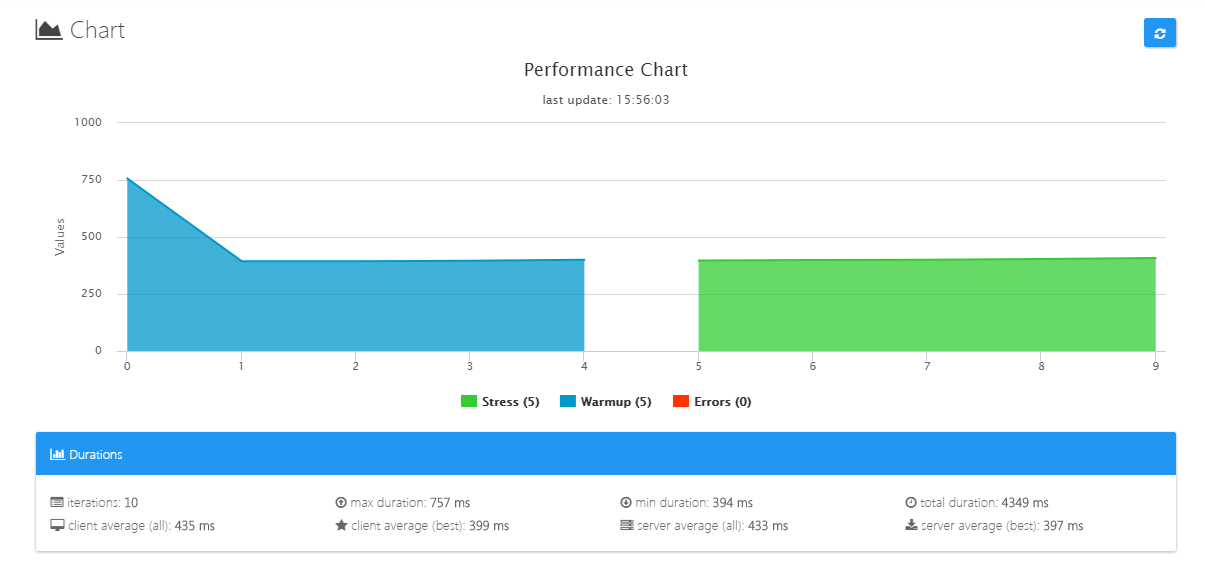
\includegraphics[scale=0.5]{Imagens/estresse10.PNG} 
  \label{estresse1}
\end{figure}

\begin{figure}[H]
  \centering
   \caption{Resultado de teste de estresse para 100 requisições.}
  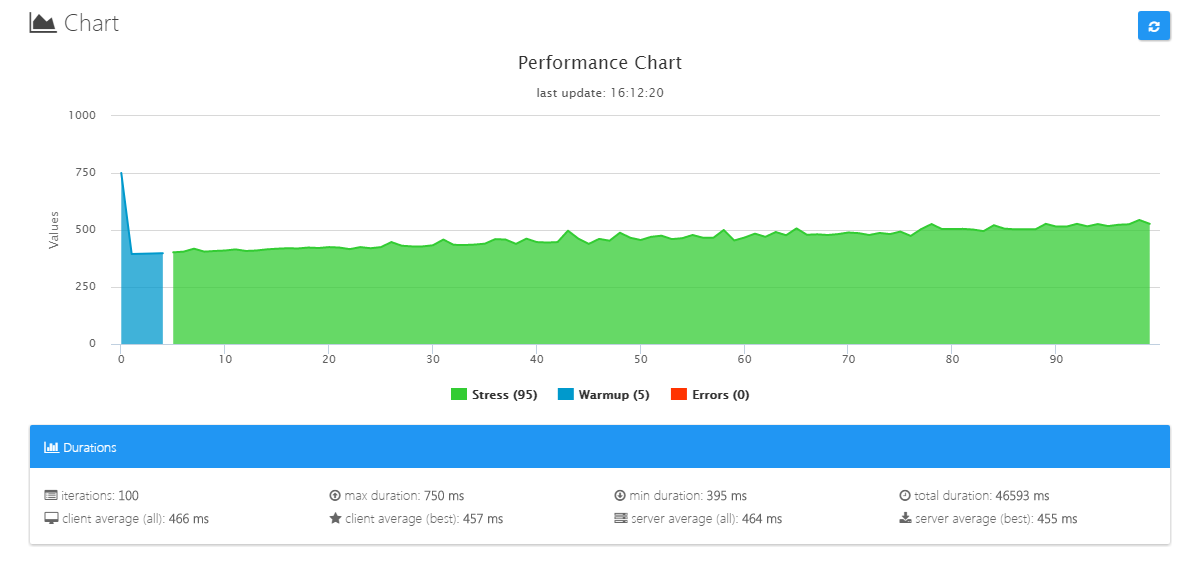
\includegraphics[scale=0.5]{Imagens/estrese100.PNG} 
  \label{estresse2}
\end{figure}

\begin{figure}[H]
  \centering
   \caption{Resultado de teste de estresse para 10 mil requisições.}
  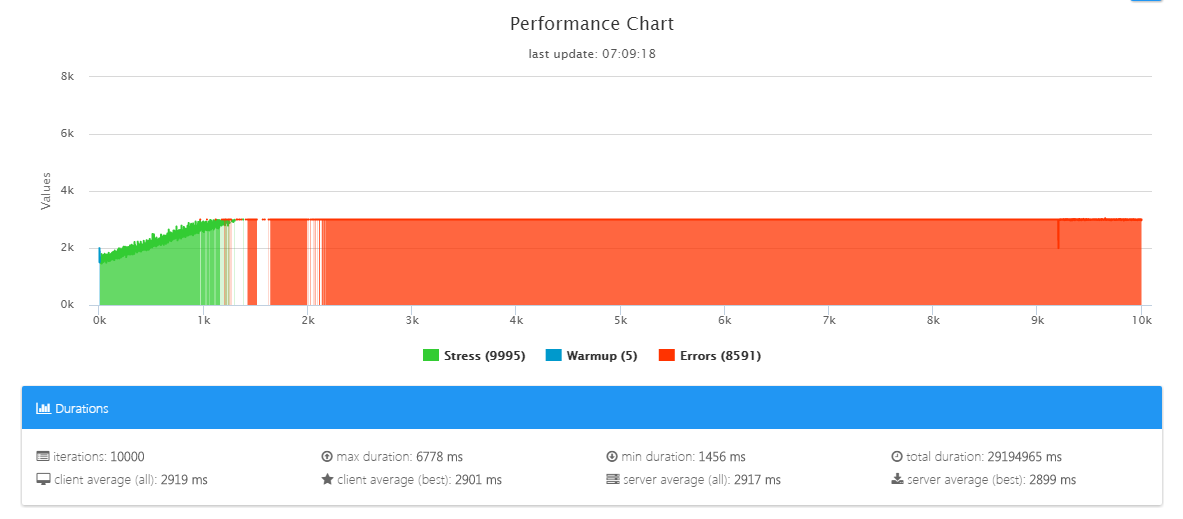
\includegraphics[scale=0.5]{Imagens/perfomance10k.PNG} 
  \label{estresse3}
\end{figure}


Para realização deste teste foi utilizada uma instância do servidor webhook executando em uma maquina virtual com as seguintes configurações:

\begin{itemize}
    \item 1GB de memória ram
    \item 25GB de disco
    \item Sistema operacional linux ubuntu 18.04 (LTS) x64 
\end{itemize}


Após a realização da tarefa dois ficou evidente que a integração de chatbots deve também levar em consideração os aspectos relacionados a escalabilidade. Ou seja, refletir sobre a hipótese do uso do software pelo usuário finais crescer e o sistema não conseguir atender as demandas. Vale ressaltar que a escalabilidade da aplicação não é um problema de integração mas de infraestrutura. Uma solução comum para realizar o gerenciamento de concorrência é realizar balanceamento de carga por meio de clusters\footnote{o termo cluster faz referência à arquitetura de sistema que une dois ou mais computadores ou aplicações como se fossem apenas um.} que possuem várias instâncias da aplicação executando. Esse é um problema que é sanado ao utilizar plataformas como Watson que possuem uma infraestrutura como serviço para os clientes.

